\documentclass[a4paper, amsfonts, amssymb, amsmath, reprint, showkeys, nofootinbib, twoside]{revtex4-1}
\usepackage[english]{babel}
\usepackage[utf8]{inputenc}
\usepackage[colorinlistoftodos, color=green!40, prependcaption]{todonotes}
\usepackage[pdftex, pdftitle={Article}, pdfauthor={Author}]{hyperref}
\usepackage{amsthm}
\usepackage{mathtools}
\usepackage{physics}
\usepackage{xcolor}
\usepackage{caption}
\usepackage{hyperref}
\usepackage{multirow}
\usepackage{amsmath}
\usepackage{amssymb}
\usepackage{graphicx}
\graphicspath{Images}
\usepackage[left=23mm,right=13mm,top=35mm,columnsep=15pt]{geometry} 
\usepackage{adjustbox}
\usepackage{placeins}
\usepackage[T1]{fontenc}
\usepackage{float}
%\usepackage{longtable}
\usepackage{csquotes}
\usepackage{refstyle}
\usepackage{lipsum}
\usepackage{booktabs}

\begin{document}

\title{ADC- DAC Circuit with Sample and Hold}
\author{Swaroop Ramakant Avarsekar}
\email{swaroop.avarsekar@niser.ac.in}
\affiliation{School of Physical Sciences, National Institute of Science Education and Research, HBNI, Jatni -752050, India}
\date{\today}


\begin{abstract}
This experiment aims to reproduce the input signal as the output by using dedicated integrated circuits for ADC and DAC circuits also sampling and holding the signal and importance of sampling frequency. We also verify the output with the theoretical formula for the case of ADC and DAC ICs. The output signal should match with that of input signal.
\end{abstract}
	
\keywords{Comparator, Ladder, Op-Amp, Sample and Hold}
	
\maketitle

\section{Theory}
ADC and DAC expands to Analog to Digital converter and Digital to Analog converter. Some of the micro-controllers work only in the digital environment, hence they cannot read analog signals but digital signals in form of 0s and 1s. DACs are used in speakers, televisions to convert digital audio / video signals to analog signals. Hence, this conversion is necessary and can be done with the ICs and resistors as follows.

 In the previous experiment, ADC and DAC circuits were constructed using LM 339, IC 7404 and IC 74147; and R-2R ladder  with IC 741, respectively. This experiment aims higher to sample the signals and holding till it is converted into digital format by ADC. Here we will be using IC 0804 for ADC and IC 0808 for DAC. 
 
 In sample and hold circuit, the signal is sampled for short interval and is held until the arrival of next input signal to be sampled. The duration of holding the sample is between ms to s.
 
 \begin{figure}[H]
 	\centering
 	\includegraphics[scale=0.2]{sh} 
 	\caption{Input and sampled signal }
 	\label{1}
 \end{figure}
\section{Experiment}
This experiment consists of four parts, as highlighted in the figure (\ref{1}) :

\begin{figure}[H]
	\centering
	\includegraphics[scale=0.3]{21} 
	\caption{Circuit diagram for ADC-DAC with sample and hold}
	\label{1}
\end{figure}

First part consists of sample and hold circuit which is constructed using IC LF398. This circuit samples the signals and holds till it is converted into digital signal. This circuit requires clock signal where it is provided by function generator.  We choose sampling frequency as 5 V, 1 kHz square from function generator and signal frequency of 100 Hz sine wave of amplitude 5 V. Use mica, polystyrene or polypropylene capacitors, refrain from using ceramic capacitors.

Second ADC circuit, The IC 0804 is an 8 bit ADC converter which will be replaced with trivial circuit. This IC also has internal clock to provide clock pulse to sample and hold circuit. This will not be used since noise is already present in the noise clock pulse signal. 
To get the digital output, we have:
\begin{equation}
	\text{Digital Output}=\frac{\text{Analog input Voltage}}{\text{Reference voltage}}\times(2^N-1)
\end{equation}

where N is the number of bits

Third part is DAC circuit, IC 0808 is an 8 bit DAC chip which is a substitute to R-2R ladder circuit. The output of this IC is given by:


\begin{equation}
	I=K\left(\frac{A_1}{2}+\frac{A_2}{4}+\frac{A_3}{8}+\frac{A_4}{16}+\frac{A_5}{32}+\frac{A_6}{64}+\frac{A_7}{128}+\frac{A_8}{128}\right) 
\end{equation}

where K=$V_{ref}/{R}$, $V_{ref}=5 V$ and R=4.7 k $\Omega$

Last part, is construction of trans impedance, which is a current to voltage converter which is constructed IC 741. This is used to process the current output of DAC circuit. We should observe that the input is reproduced as the output. 

\section{Observations}
\begin{figure}[H]
	\centering
	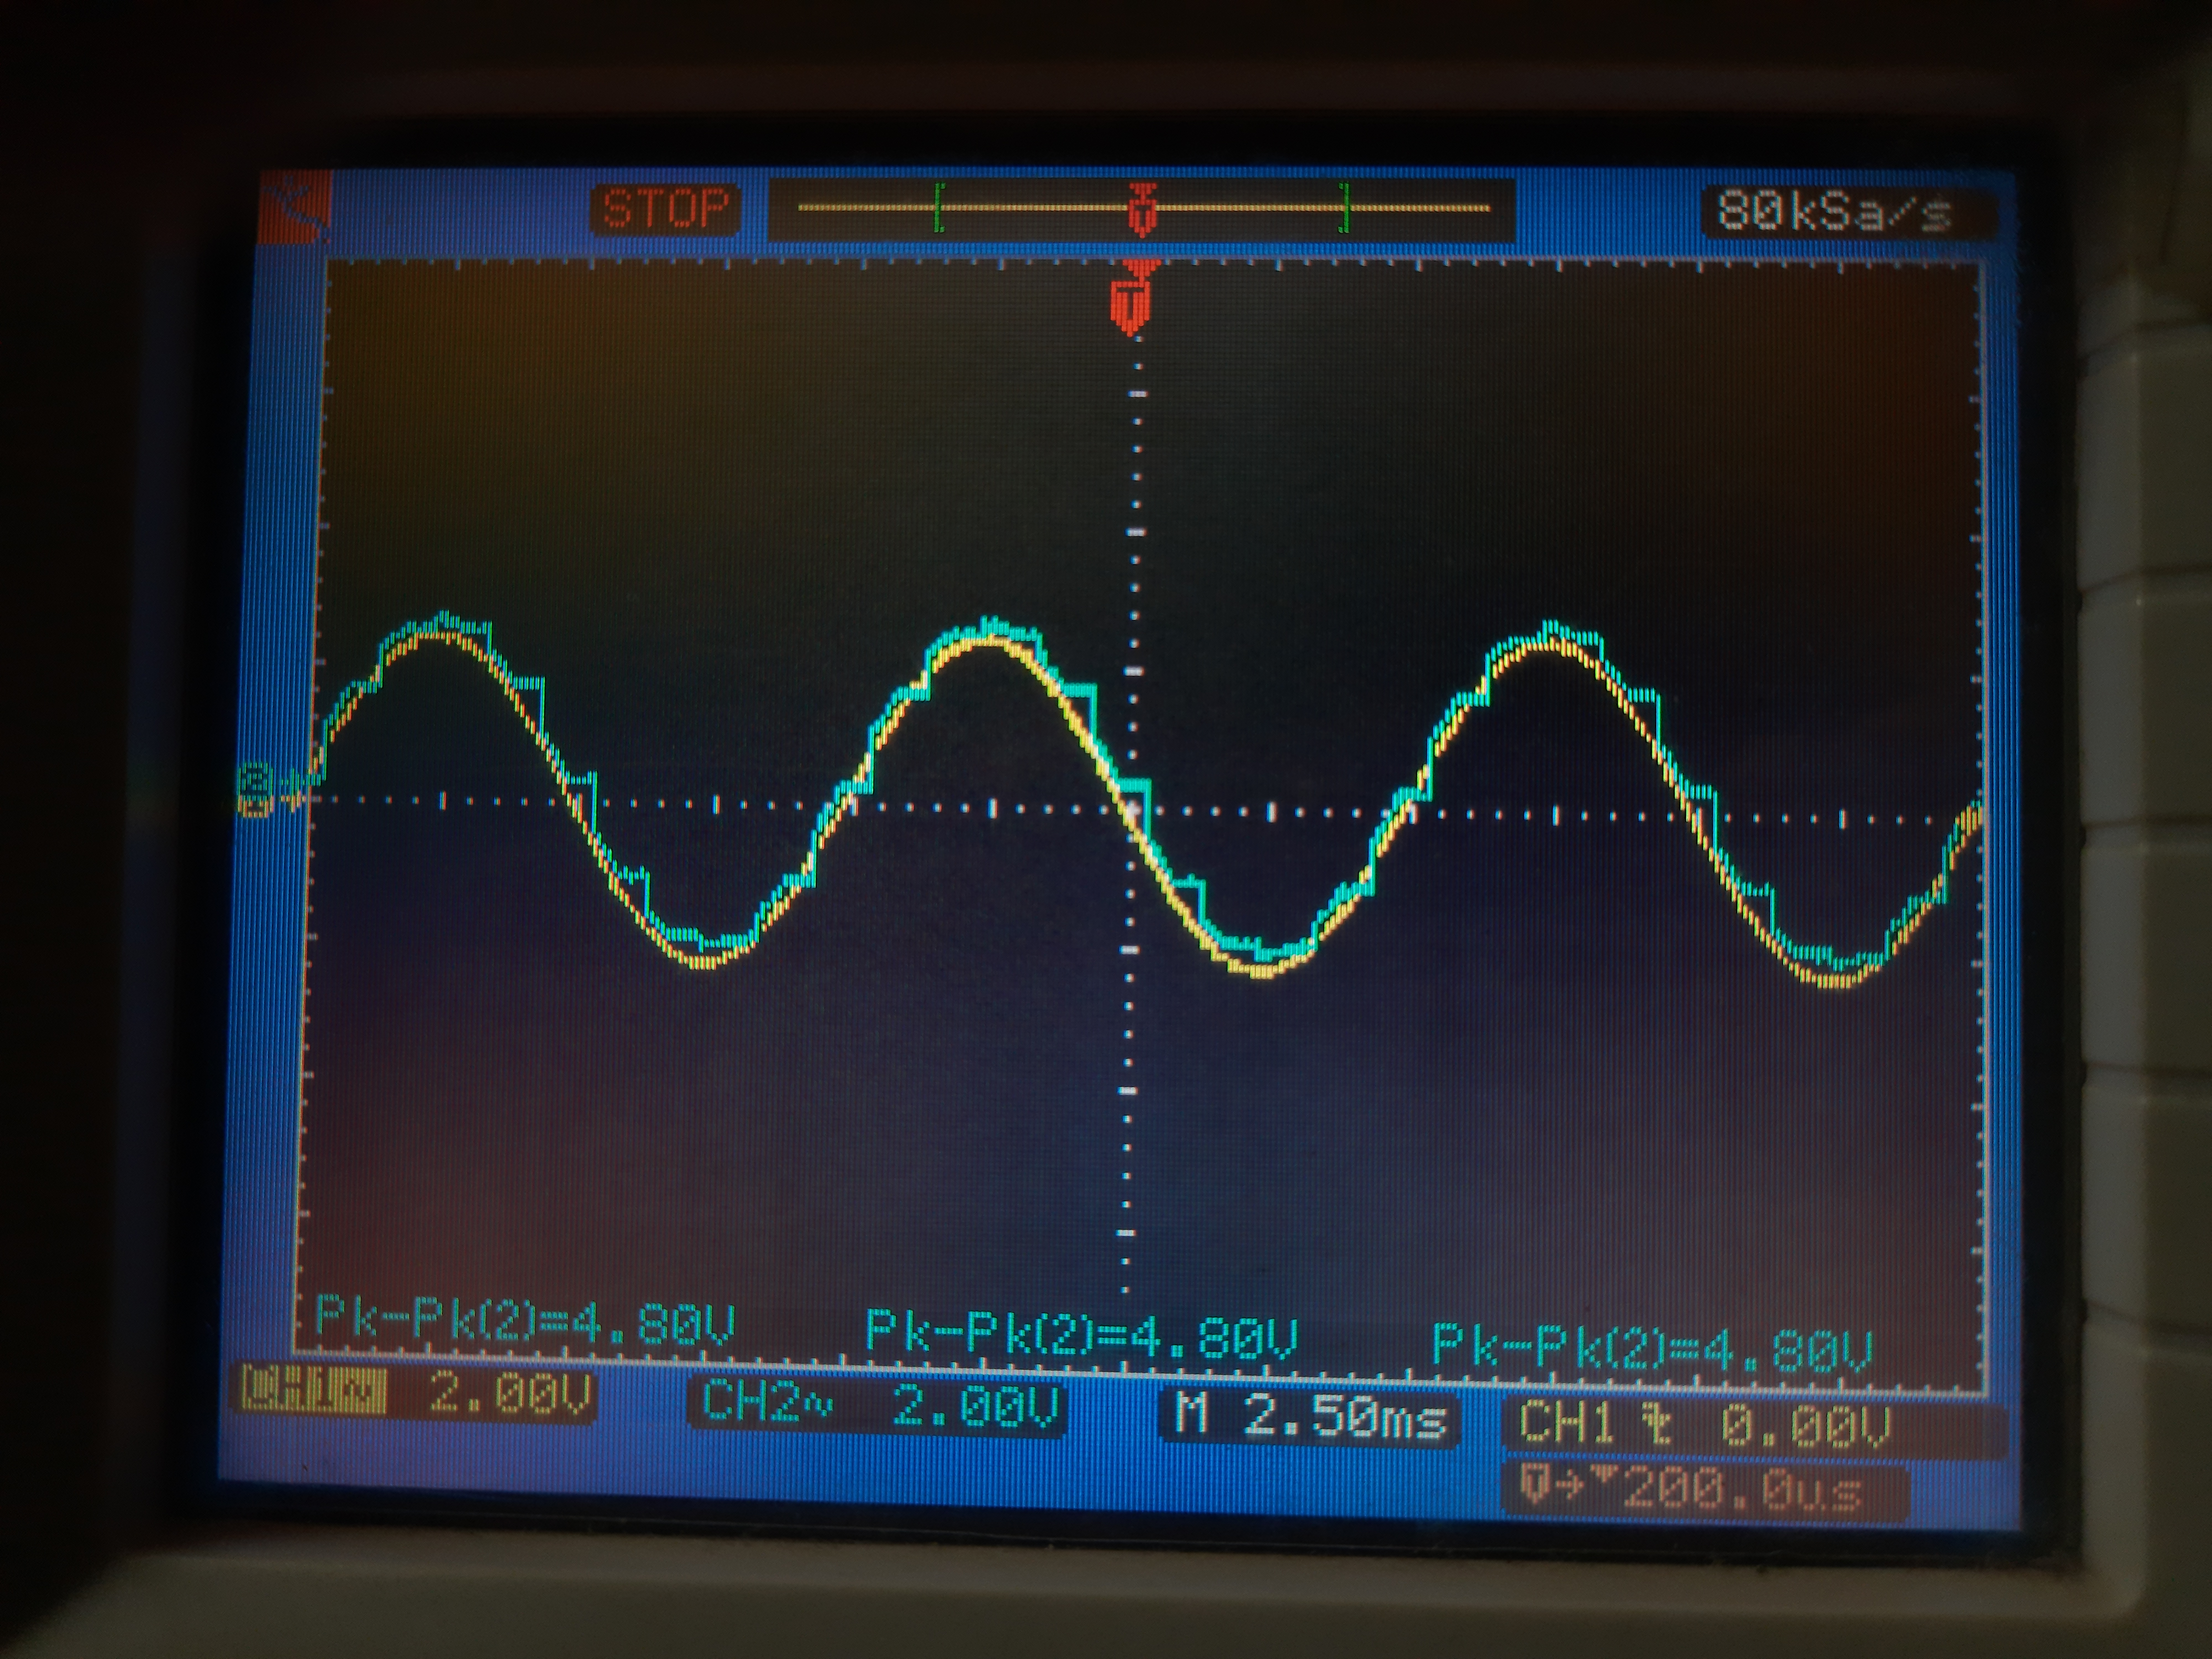
\includegraphics[scale=0.025]{s} 
	\caption{Oscilloscope display during sampling and holding the signal}
	\label{s}
\end{figure}

Sinusoidal wave is input signal with sampling signal to be 5V peak to peak 1 kHz square wave signal. 

\begin{table}[H]
	\centering
	\caption{ADC (Analog to Digital) Circuit verification}
	\label{t1}
	\resizebox{\columnwidth}{!}{%
		\begin{tabular}{|c|c|c|c|c|c|}
			\hline
			\begin{tabular}[c]{@{}c@{}}Sl \\ No.\end{tabular} &
			\begin{tabular}[c]{@{}c@{}}Input DC\\ Voltage (V)\end{tabular} &
			\begin{tabular}[c]{@{}c@{}}Binary \\ Output\end{tabular} &
			\begin{tabular}[c]{@{}c@{}}Calculated DC\\ using equation\end{tabular} &
			\begin{tabular}[c]{@{}c@{}}Binary \\ to Analog\end{tabular} &
			\begin{tabular}[c]{@{}c@{}}Error \\ (\%)\end{tabular} \\ \hline
			1 & 0.918 & 110001   & 46.818  & 49  & 4.660600624 \\ \hline
			2 & 1.276 & 1000100  & 65.076  & 68  & 4.493207941 \\ \hline
			3 & 2.056 & 1101101  & 104.856 & 109 & 3.952086671 \\ \hline
			4 & 2.266 & 1111000  & 115.566 & 120 & 3.8367686   \\ \hline
			5 & 3.241 & 10101100 & 165.291 & 172 & 4.058902179 \\ \hline
			7 & 3.706 & 11000101 & 189.006 & 197 & 4.22949536  \\ \hline
			6 & 4.02  & 11010101 & 205.02  & 213 & 3.89230319  \\ \hline
			8 & 4.85  & 11111111 & 247.35  & 255 & 3.092783505 \\ \hline
		\end{tabular}%
	}
\end{table}

The average percentage for ADC is error is 4.02\%.

\begin{table}[H]
	\centering
	\caption{DAC (Digital to Analog) Circuit verification					}
	\label{t2}
	\resizebox{\columnwidth}{!}{%
		\begin{tabular}{|r|r|r|r|r|}
			\hline
			\multicolumn{1}{|l|}{\begin{tabular}[c]{@{}l@{}}Sl \\ No.\end{tabular}} &
			\multicolumn{1}{l|}{\begin{tabular}[c]{@{}l@{}}Binary \\ Input\end{tabular}} &
			\multicolumn{1}{l|}{\begin{tabular}[c]{@{}l@{}}Calculated DC \\ Voltage (V)\end{tabular}} &
			\multicolumn{1}{l|}{\begin{tabular}[c]{@{}l@{}}Measured DC\\ Voltage (V)\end{tabular}} &
			\multicolumn{1}{l|}{Error (\%)} \\ \hline
			1 & 11111111 & 5            & 5.18  & 3.6         \\ \hline
			2 & 1111111  & 2.490196078  & 2.653 & 6.537795276 \\ \hline
			3 & 111111   & 1.235294118  & 1.385 & 12.11904762 \\ \hline
			4 & 1011111  & 1.862745098  & 1.976 & 6.08        \\ \hline
			5 & 11111    & 0.6078431373 & 0.658 & 8.251612903 \\ \hline
			6 & 1111     & 0.2941176471 & 0.32  & 8.8         \\ \hline
			7 & 10011111 & 3.117647059  & 3.326 & 6.683018868 \\ \hline
			8 & 11011111 & 4.37254902   & 4.7   & 7.488789238 \\ \hline
		\end{tabular}%
	}
\end{table}

The average percentage for DAC is error is 7.44\%.

\section{Conclusion}
In this experiment we have constructed the sample and hold circuit with sinusoidal signal as input signal and square wave as sampling signal. We also verified the output of ADC and DAC ICs, i.e 0804 and 0808 giving the percentage error as 4.02\% and 7.44\%. The trans-impedance amplifier was constructed using IC 741 which was used to measure the voltage readings from the output of IC 0808. The individual components were successful and worked independently and completed the circuit by connecting these components and input was reproduced at the output.

The majority of errors encountered during the experiment may have been the result of several factors. These could include issues with the power supply, such as inconsistent or insufficient voltage, as well as problems with the bias voltage, which may have been set incorrectly or varied in an unpredictable manner. Another potential source of error may have been the use of faulty multi-meters, which could have provided inaccurate readings or failed to function properly. Loose connections between components on the breadboards may have caused intermittent or inconsistent signals, leading to incorrect measurements. Finally, improper grounding between the breadboards may have also contributed to errors by allowing unwanted electrical interference or noise to affect the readings.

\section{References}
SPS manual, www.tek.com, www.electronicshub.org

\end{document}